In this section we outline our approach for recreating the DeepXSS architecture, including difficulties we had in reproducibility, limitations with DeepXSS that needed to be addressed, some creative liberties we took, and a few alternative machine learning architectures that proved interesting. 

\subsection{Data Preprocessing}
\subsubsection{Decoding}
We built a custom recursive URL decoder. This decoder performs a depth first search of 5 different decodings. At each level, the decoder tries to decode the URL with all decodings, for each decoding that is successfull, the decoder will recursively try to further decode the string that resulted from the decoding; see algorithm \ref{decoder} for a pseudocode implementation. The first string enoucountered that none of the decoders can decode is returned as the decoded string. The supported encodings are: URL unicode encoding (this includes characters of the form \%uxxxx and \textbackslash uxxxx),URL encoding (that is characters of the form \%xx), HTML character references (that is characters of the form \&xx;), hex encoding, and base64 encoding. 

Algorithm \ref{decoder} works as follows: on line \ref{dec:all} all the decoder functions are called and passed the URL to be decoded. These functions all return a Tuple of the form (Boolean, String) where the Boolean value indicates if the decoding was successfull while the String is the decoded string (the String remains unchanged if the decoding fails). Next, on line \ref{dec:res}, the result tuples of all the attempted decoders are looped over. If it's found that a decoder was successful (line \ref{dec:check}) then recurisvely call the decoder on the resulting string (line \ref{dec:rec}). If the recursive decoding succeeds than return the result of the recursive call (\ref{dec:rec:true}). If the decoder gets to line \ref{dec:nrec}, than that means one of two things happened: either none of the decoders succeeded, in which case the string must be fully decoded and so we go to line \ref{dec:true}; if on the other hand some of the decoders succeeded, then if the algorithm gets to line \ref{dec:nrec} it must have been the case that none of the recursive calls succeeded (meaning line \ref{dec:rec:true} was never reached) which means the decoder was unable to decode the string and we return on line \ref{dec:false}. 

\begin{algorithm}
\caption{Recursive Decoder}\
\label{decoder}
\begin{algorithmic}[1]
    \Function{decode}{url}
        \State decoders $\gets$ [url(), unicode(), html(), hex(), base64()]
        \State dec\_results $\gets$ []
        \For{decoder \textbf{in} decoders} \label{dec:all}
            \State dec\_results.append(decoder(url))
        \EndFor

        \State some\_decoded $\gets False$
        \For{decode\_success, decode\_str \textbf{in} dec\_results} \label{dec:res}
            \State some\_decoded $\gets$ decode\_success \textbf{or} some\_decoded
            \If{decode\_success} \label{dec:check}
                \State (next\_decode\_success, next\_decode\_str) = DECODE(decode\_str) \label{dec:rec}
                \If{next\_decode\_success}
                    \State \Return ($True$, next\_decode\_str) \label{dec:rec:true}
                \EndIf
            \EndIf 
        \EndFor

        \If{some\_decoded} \label{dec:nrec}
            \State \Return ($False$, url) \label{dec:false}
        \Else 
            \State \Return ($True$, url) \label{dec:true}
        \EndIf

    \EndFunction
\end{algorithmic}
\end{algorithm}

To clarify with an example, consider the URL:

\urlline{http://example.com/706174682F746F2F66696C653F783D26616D703B6C743B73637269707426616D703B67743B253230616C65727428253230312532302925323026616D703B6C743B2F73637269707426616D703B67743B}. 

Passing this through the decoder, the Hex decoder will succeed and produce the string: 

\urlline{http://example.com/path/to/file?x=\&amp;lt;script\&amp;gt;\%20alert(\%201\%20)\%20\&amp;lt;/script\&amp;gt;} 

then the URL decoder will succeed giving the string: 

\urlline{http://example.com/path/to/file?x=\&amp;lt;script\&amp;gt; alert( 1 ) \&amp;lt;/script\&amp;gt;}

then the HTML decoder will succeed and give:

\urlline{http://example.com/path/to/file?x=\&lt;script\&gt; alert( 1 ) \&lt;/script\&gt;} 

and finally the HTML decoder will succeed again and give: 

\urlline{http://example.com/path/to/file?x=<script> alert( 1 ) </script>}. 

No decoders will succeed here making this the final form.


\subsubsection{Tokenization}
As seen in table \ref{tok:tab}, DeepXSS defined six different token types. We expanded on this set of tokens and ended up with a total of 14 token types. The reason we expanded on this token set is because many URLs contained zero tokens. For example \url{http://www.wittebeer.be/?oid=911\&pid=8056} or \url{http://www.facebook.com/Euphnet?sk=wall}, both of which are in the DMOZ directory, do not contain any of their token types. Using more token types common to normal URLs and increasing the feature richness as a way to have benign samples not be empty was something we encountered in the literature \cite{mokbal2019mlpxss}\cite{zhang2019cross}. But put basically, we didn't want our classifier to come to learn that benign URLs are largely empty; we wanted it to learn the structure of both benign and malicious URLs. As such, we expanded their table to include 8 more as shown in table \ref{exp:tok:tab}.


\begin{table}
\begin{center}
\begingroup
\setlength{\tabcolsep}{5pt} % Default value: 6pt
\renewcommand{\arraystretch}{1.5} % Default value: 1
\begin{tabular}{||c | c||} 
    \hline
    Classification & Example \\ [0.5ex] 
    \hline\hline
    \textbf{Integer Argument} &  (543), (1), (2004) \\ 
    \hline
    \textbf{Integer Constant} &  1, 2, 5432, 54 \\ 
    \hline
    \textbf{String Argument} & (``Hello''), (String.fromCharCode(65)) \\
    \hline
    \textbf{Assignment LHS} & x=, variable= \\
    \hline
    \textbf{Assignment RHS} & =x, =654, =value \\
    \hline
    \textbf{Path} & path/ t56543-trer-yt43/ \\ 
    \hline
    \textbf{Identifier} & iden, value, hello, goodbye \\ [1ex] 
    \hline
\end{tabular}
\endgroup
\caption{\label{exp:tok:tab}Extended DeepXSS Tokens.}
\end{center}
\end{table}

An integer argument token is any integer value that follows a function name token and is enclosed in brackets. Similarly, a string argument token is taken to be any argument that isn't an integer; hence \textit{String.fromCharCode(65)} being an example of a string argument. We figured that distinguishing futher between arguments would be superfluous, and by inspection these were the most common arguments (including functions which returned a string or integer). The integer constant token was introduced because many URLs contained non-descript integers outside of function calls and URL arguments. The two assignment tokens (left-hand side and right-hand side) were introduced so that URL arguments would not be lost (notice that the two benign examples include arguments that are skipped by DeepXSS). Similarly, path tokens were intoduced so that the path wasn't entirely skipped. And finally we introduced a generic identifier token. Assignment LHS, Path, Script URL, Function Name, and Windows Events all begin with an identifier but all have additional characters to further distinguish them (for example Windows Events always start with `on' and end with `=', paths end with `/' or `?', etc). Any identifier that is found that cannot be further categorized is included as a generic Identifier token.

\subsubsection{Generalization}
In keeping with DeepXSS, we generalized many parts of the URL. In the original paper all the domains became simply `website'. Having every URL begin with `http://website' communicates no information and so we simply ommitted the domain. We mapped all integer arguments to `(1)' and all string arguments to `(``str\_arg'')'. All integer constants were mapped to `1'. The left-hand side of assignments were all generalized to `assign<num>=' where `<num>' starts from 0 and increments for each encountered left-hand side. This was done because most identifiers in URLs proved to be unique, and so not useful in classification (especially when using CBOW) with the exception of Function Names, script URLs, and Windows Events which are reserved words and so can't be unique across many URLs. The right-hand sides are generalized to `val<num>' where `<num>' again increments with each right-hand side encountered. Similarly, all path tokens are generalized to `path<num>/' and finally all identifier tokens were mapped to `ident<num>'.

To clarify the tokenization and generalization process with an example, consider \urlline{http://website/search.php?uid=ws848d8024088c327.36898031\&src=\&term=<script>alert(123)</script>\&args=qs=06o}. The following sequence of (token type, token value) pairs would be extracted going left to right:

\begin{enumerate}
\item \texttt{(Path, `path0/')} for \url{search.php?}
\item \texttt{(Assignment LHS, `assign0=')} for \texttt{uid=}
\item \texttt{(Assignment RHS, `val0')} for \texttt{=ws848d8024088c327}
\item \texttt{(Integer Constant, 1)} for \texttt{36898031}
\item \texttt{(Assignment LHS, `assign1=')} for \texttt{src=}
\item \texttt{(Assignment LHS, `assign2=')} for \texttt{term=}
\item \texttt{(Start Label, `<script>')} for \texttt{<script>}
\item \texttt{(Function Name, `alert')} for \texttt{alert(}
\item \texttt{(Integer Argument, `(1)')} for \texttt{(123)}
\item \texttt{(End Label, `</script>')} for \texttt{<script>}
\item \texttt{(Assignment LHS, `assign3=')} for \texttt{args=}
\item \texttt{(Assignment LHS, `assign4=')} for \texttt{qs=}
\item \texttt{(Integer Constant, `06')} for \texttt{06}
\item \texttt{(Identifier, `o')} for \texttt{o}
\end{enumerate}

Note that if two different token types overlap, the one that starts earlier is preferred; if they start in the same place then the one that extends further is preferred. This is why `args=qs=' is taken to be two left-hand sides--the `qs' could be a right-hand side, but with the equals on the right its taken to be a left-hand side since that is longer and both start at the `q'. As per the last two tokens, identifiers cannot start with numbers  (in Javascript) and so the 06o is taken to be an integer constant followed by an identifier.


\subsection{Word2Vec}

As one of the primary stated contributions of the original DeepXSS \cite{fang2018deepxss} paper, properly implementing CBOW for Word2Vec is an important part of our recreation. Unfortunately, the authors do not give good indication as to how CBOW was applied, merely stating that CBOW was used to construct word representations. We therefore took liberties with our implementation and based many decisions on the work from \cite{afzal2021deeplearning}. One major point of confusion was whether CBOW representations were constructed for token type labels, or the token itself. To test the difference, we implemented both.

In order to generate the CBOW embeddings we first needed to build a vocabulary of tokens with each token represented by a unique integer. Zeros represent padding tokens which are used later in the process.  Once the vocabulary is constructed, each list of URL tokens is replaced with corresponding integer representations.  Every vectorized URL is then padded with zeros until they are all a uniform length.  The padding tokens ensure that empty space does not influence the outcomes of the model.
Fig. 1 shows the architecture for the model we use to generate our CBOW embeddings.  For every token in our vectorized URL, the CBOW model attempts to predict the current token using the tokens around it.  Using a window size of two means that our CBOW model will attempt to predict the middle token using two adjacent tokens on either side of it.  As the model does this for every token in the dataset, the weights of the embedding layer are trained.  The embedding layer is responsible for taking each token and turning it into a multidimensional representation.  In the case of token type labels, each token will have a ten-dimensional representation and token values receive a 50-dimensional representation.

\begin{figure}[H]
    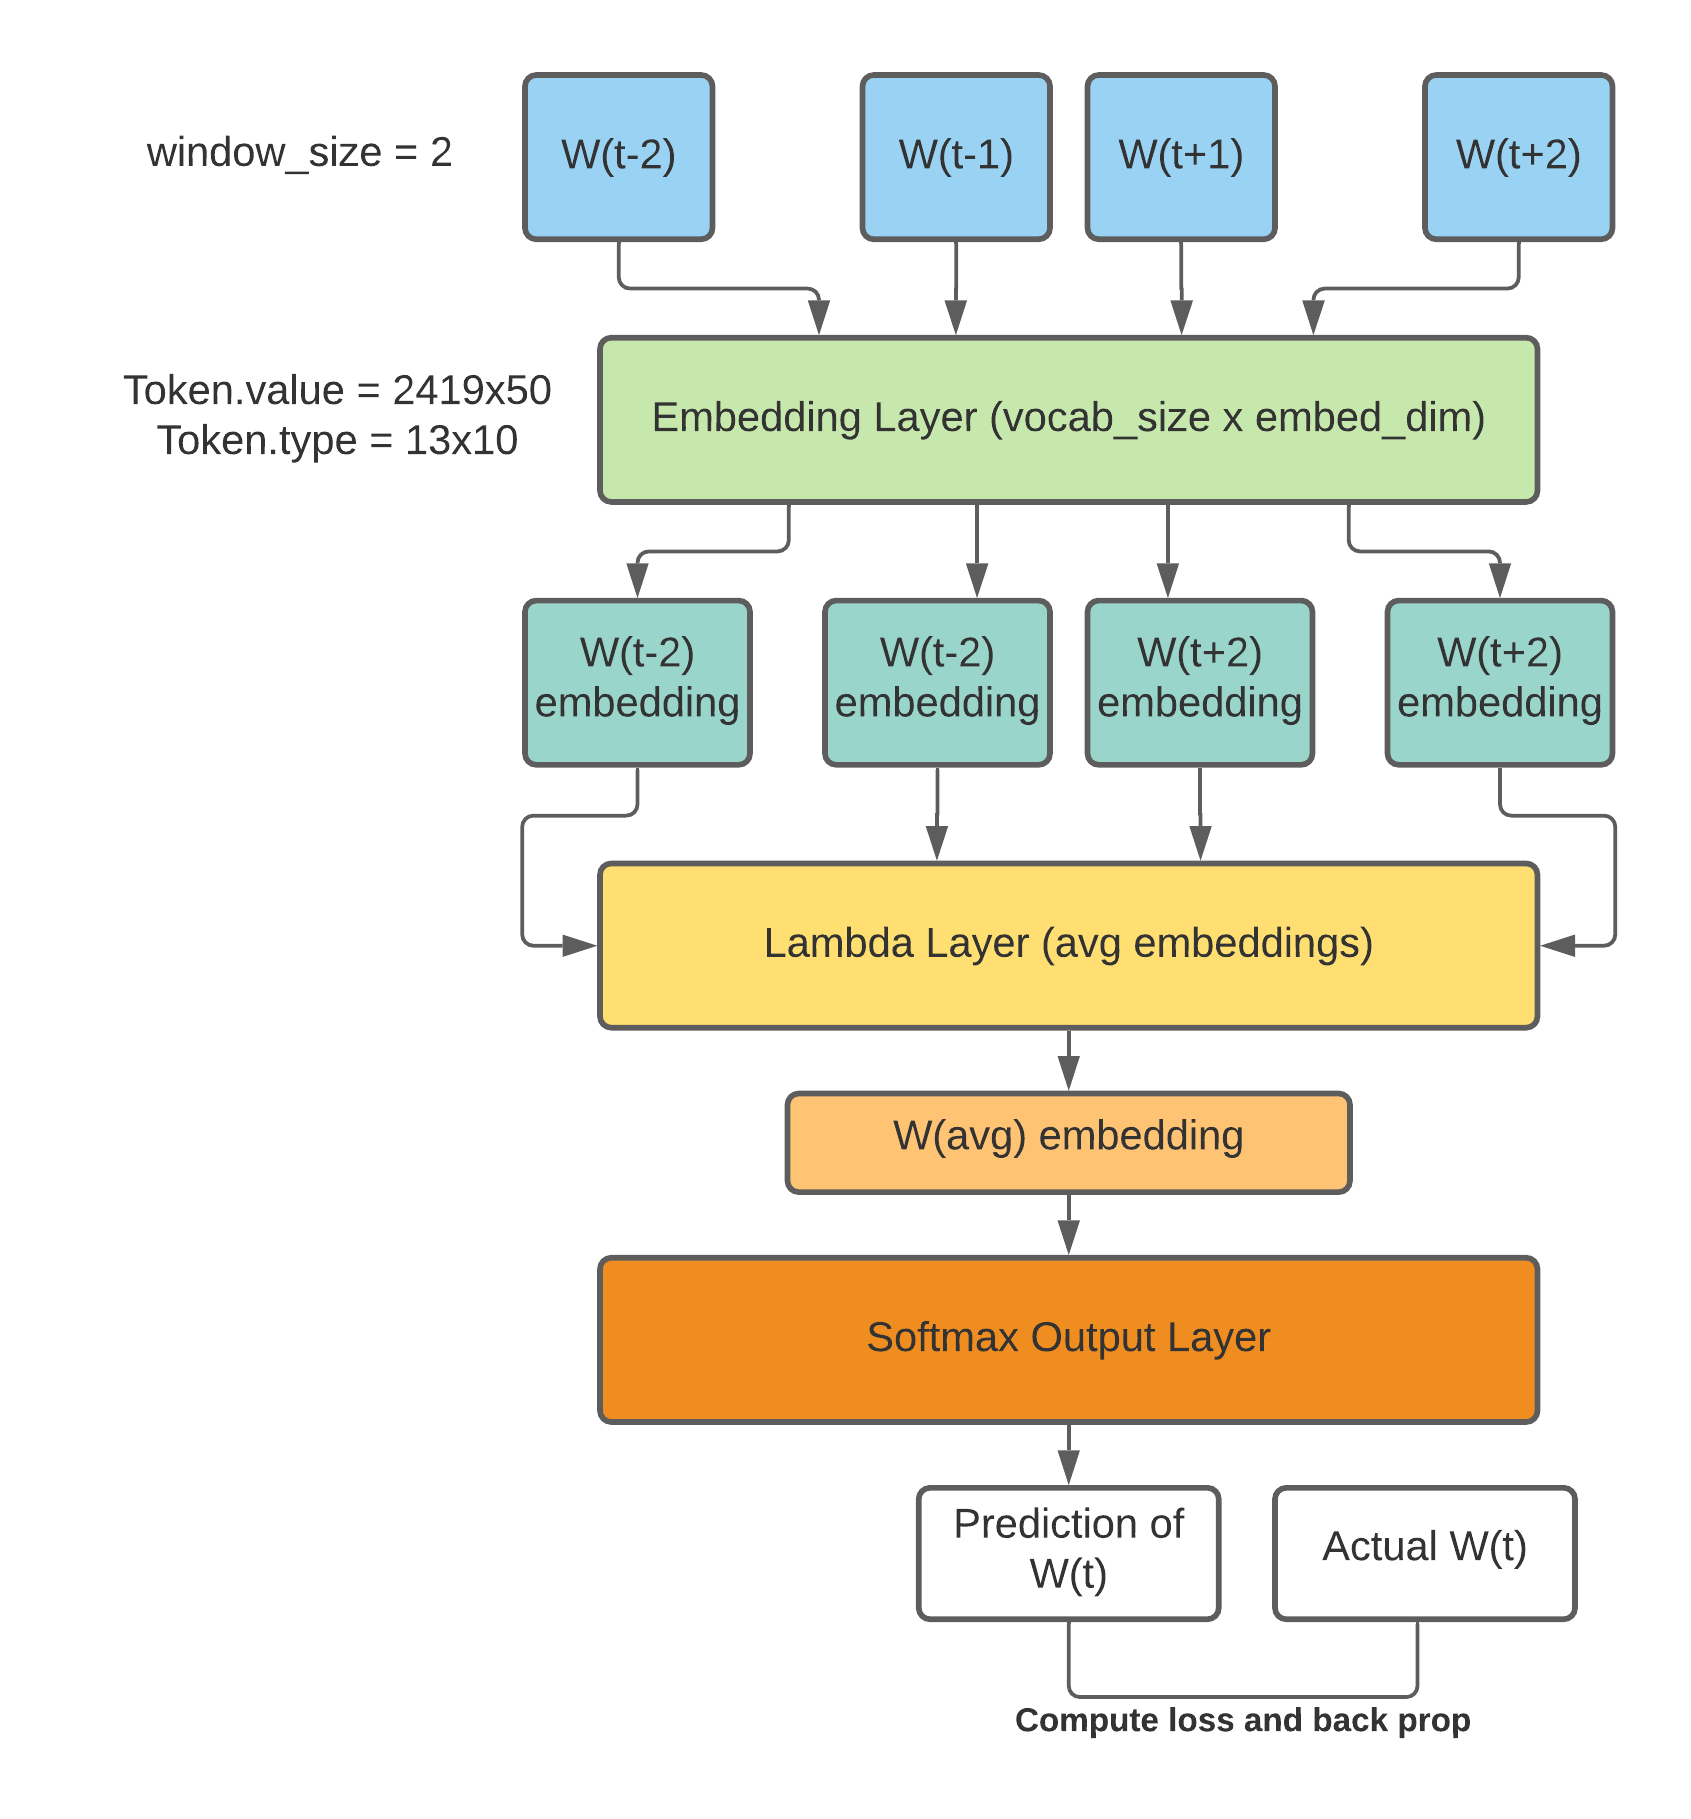
\includegraphics[width=0.45\textwidth, angle=0]{cbow_model}
\end{figure}

\begin{lstlisting}[caption=Related token values, label=cbow-exp-value]
<script>: >,ident1,</title>,path4/,<h1>
alert: ident11,ident13,ident12,<img>,path4/
</script>: <h1>,<marquee>,ident2,ident4,ident5
(1): ident4,<"<<script>,javascript,</style>,</title>
path0/: assign0=,ident1,ident0,</title>,<iframe>  
\end{lstlisting}


\begin{lstlisting}[caption=Related token types, label=cbow-exp-type]
path: int_const,value,int_arg,func_name,assign
int_const: path,value,assign,func_name,int_arg
assign: value,other,int_cons,int_arg,str_arg
value: assign,other,int_const,int_arg,func_name
ident: other,start_label,value,assign,int_arg  
\end{lstlisting}

Extracting the weights from the embedding layer and calculating the Euclidean distance between tokens allows us to see an example of similar words according to our CBOW embeddings.  Fig. 2 shows examples of the five most closely related tokens for both token value and token type.

Training each new CBOW model on the entire dataset could take as many as 24 hours meaning we needed to make changes to the tokenization process to produce better generalized data.  This sped up CBOW generation but likely resulted in some lost semantic information.


\subsection{LSTM Classifier}

The final stated contribution of DeepXSS \cite{fang2018deepxss} and arguably the most important is the LSTM classifier for XSS detection.  The authors provide a brief description of this classifier stating that it has three layers: an LSTM layer, a dropout layer to reduce overfitting, and a softmax output layer that makes predictions.  We had two primary difficulties in reconstructing the model from this description.

The first difficulty was with using the embedded token vectors in the LSTM.  We often had large numbers of embedded token vectors for every URL.  This resulted in large, nested arrays of data that were difficult to work with. We chose to transplant a non-trainable embedding layer from our CBOW model into the LSTM model as shown in \ref{lstm_model}.  This allows us to simply feed the model sequences of integers where the embeddings are constructed within the model rather than during preprocessing.

\begin{figure}[H]
	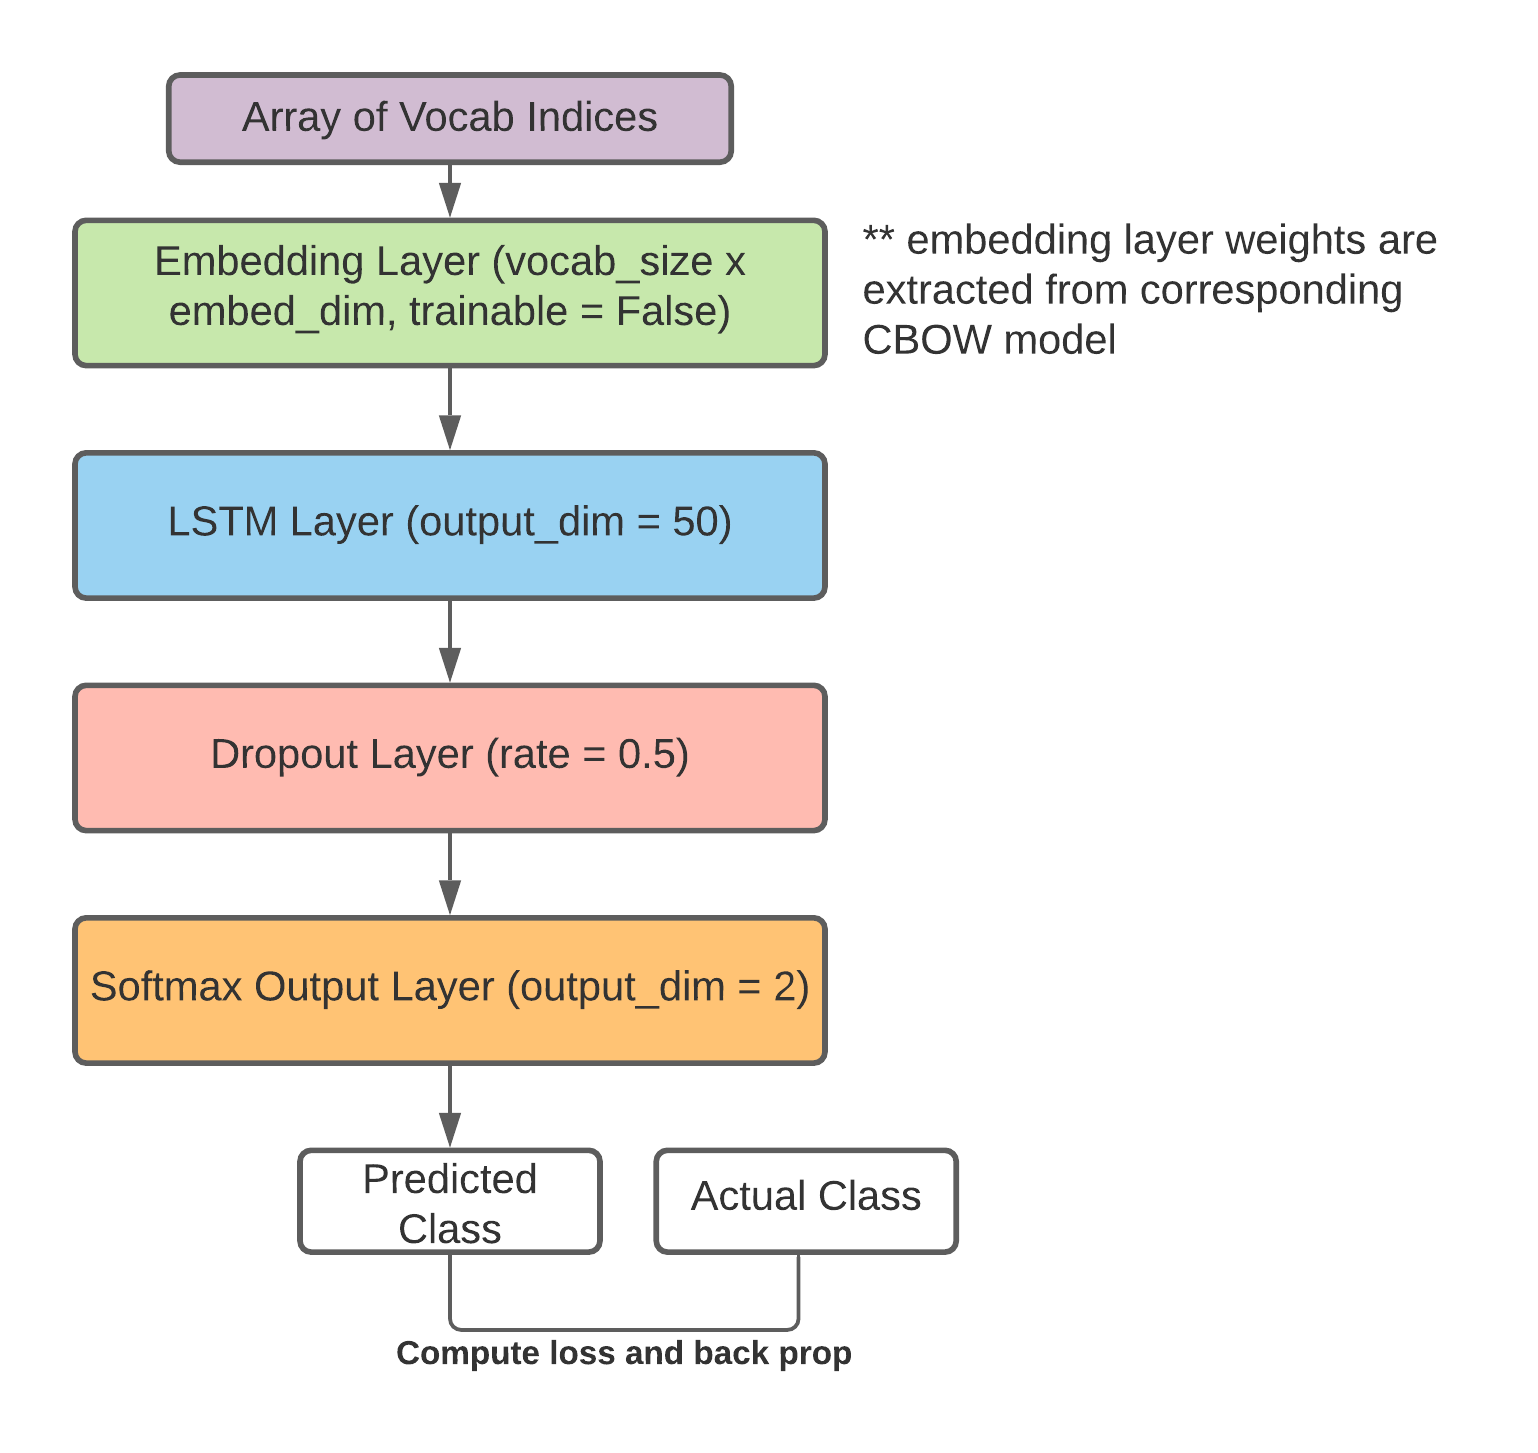
\includegraphics[width=0.8\textwidth, angle=0]{lstm_model}
\end{figure}

The other difficulty we had with constructing and training the LSTM model was with hyperparameters and model details. We found that the LSTM was often very difficult to train, seemingly making no progress after multiple epochs.  Experimenting with dropout rates, the output size of the LSTM, and several other factors was extremely time consuming.  Eventually we were able to settle on the model in \ref{lstm_model} as our primary architecture for both token type and token value.

We also constructed other models to test the importance of various design choices from the original DeepXSS paper \cite{fang2018deepxss}.  The first model is our primary design that is shown in \ref{lstm_model}. We also created a model with a sigmoid output layer, given that a softmax output layer is somewhat unnecessary for a dual classification model.  Another model is intended to test the value of the CBOW embeddings by simply training the model on sequences of integers that map to all of the tokens.  This model has no embedding layer.  The final model has an untrained embedding layer to test if the CBOW needed to be performed separately or if word embeddings could be learned through normal training.  All of these models exist for both token type and token value resulting in eight models total.  The models are listed in \ref{model-sum}.



\begin{table}
\begin{center}
\begingroup
\setlength{\tabcolsep}{6pt} % Default value: 6pt
\renewcommand{\arraystretch}{1.5} % Default value: 1
\begin{tabular}{|| c | c | c | c ||} 
    \hline
    Model & Output & Embedding & Input \\ 
    \hline\hline
    \textbf{Value-Softmax} & softmax & CBOW & Token values \\
    \hline
    \textbf{Value-Sigmoid} &  sigmoid & CBOW & Token values \\ 
    \hline
    \textbf{Value-Sequential} & softmax & None & Token values \\
    \hline
    \textbf{Value-Random} & softmax & Random & Token values \\
    \hline
    \textbf{Type-Softmax} & softmax & CBOW & Token types \\
    \hline
    \textbf{Type-Sigmoid} & sigmoid & CBOW & Token types \\
    \hline
    \textbf{Type-Sequential} & softmax & None & Token types \\
    \hline
    \textbf{Type-Random} & softmax & Random & Token types \\
    \hline
\end{tabular}
\endgroup
\caption{\label{model-sum}Summary of Models}
\end{center}
\end{table}
